\documentclass[a4paper,11pt,fleqn]{article}
\usepackage{podes-template}

%pacotes adicionais
\usepackage[linesnumbered, algoruled, vlined, portuguese]{algorithm2e}
\usepackage{listings}
\lstset
{ %Formatting for code in appendix
	language=Python,
	numbers=left,
	stepnumber=1,
	showstringspaces=false,
	tabsize=1,
	breaklines=true,
	breakatwhitespace=false,
	extendedchars=true,
	literate={á}{{\'a}}1 {õ}{{\~o}}1 {ã}{{\~a}}1 {í}{{\'i}}1 {é}{{\'e}}1 {ç}{{\,c}}1,
}

%%%%%%%%%%%%%%%%%%%%%%%%%%%%%%%%%%% %%%%%%%%%%%%%%%%%%%%%%%%%%%%%%%%%%%%%%%


%título do artigo
\title{Desenvolvendo Resolvedores de Programação Linear Inteira Mista em Python usando o pacote Python-MIP$^1$} 

%define os autores
\author{
 \name{Haroldo G. Santos\authortag{a}\corresponding{haroldo@ufop.edu.br}}, 
 \name{Túlio A.M. Toffolo\authortag{a}} \\
 \authortag{a}
 \institute{Instituto de Ciências Exatas e Biológicas, Departamento de Computação\\ Universidade Federal de Ouro Preto, Ouro Preto, MG, Brasil}
}

\authorrunning{Santos \& Toffolo}


\begin{document}


\maketitle


\begin{resumo}
O pacote Python-MIP oferece um conjunto abrangente ferramentas para a modelagem e resolução de Problemas de Programação Inteira Mista em Python. Além de oferecer uma linguagem de modelagem de alto nível, o pacote permite o desenvolvimento de resolvedores avançados, habilitando comunicação bidirecional com o resolvedor durante o processo de busca. Neste tutorial desenvolveremos resolvedores de Programação Linear Inteira Mista para o Problema do Caixeiro Viajante. Iniciando com um resolvedor simples baseado em uma formulação compacta iremos evoluir para um resolvedor que combina heurísticas e planos de corte para a resolução eficaz de problemas de grande porte.

\end{resumo}

\begin{palavras}
Otimização Combinatória, Caixeiro Viajante, Programação Linear Inteira, Python.
\end{palavras}

\begin{abstract}
The Python-MIP package offers a comprehensive set of tools for the modeling and solution of Integer Linear Programming Problems in Python. Besides providing a high level modeling language, the package allows the development of advanced solvers with di-directional communication with the solver during the search process. In this tutorial we develop solvers for the Traveling Salesman Problem. Starting with a simple solver based on a compact formulation we evolve to a solver combining heuristics and cutting planes for the effective solution of large scale instances.
\end{abstract}

\begin{keywords}
Combinatorial Optimization, Traveling Salesman Problem, Integer Linear Programming, Python. 
\end{keywords}


\newpage
\thispagestyle{defaultPage}

Python-MIP é um pacote para modelagem e resolução de Problemas de
Programação Linear Inteira Mista (PLIM) \citep{Wolsey1998} em Python.
O projeto do pacote foi feito com o objetivo de desenvolver uma ferramenta
que atendesse os seguintes requisitos:

\begin{enumerate}
	\item clareza de código e modelagem de alto nível
	\item alto desempenho
	\item extensibilidade e configurabilidade
\end{enumerate}

Tradicionalmente, os objetivos 1 e 2 foram considerados conflitantes.
Até recentemente, as opções mais recomendada para os interessados
em 1 eram linguagens algébricas de alto nível como AMPL \citep{Fourer1987}.
A obtenção de desempenho máximo costumava requerer o uso de linguagens
de mais baixo nível como C \citep{Johnson1991a}. Resolvedores estado-da-arte
como o CPLEX foram escritos nessa linguagem \citep{Bixby2002}. Desse
modo, a biblioteca completa de funções estava originalmente 
disponível somente nela. Recentemente, soluções como JuMP\citep{Dunning2015}
demonstraram que os objetivos 1 e 2 não são necessariamente conflitantes:
linguagens de alto nível como Julia juntamente com compiladores \emph{just-in-time}
permitem o desenvolvimento rápido de resolvedores que apresentam alto
desempenho. O objetivo do projeto Python-MIP é o desenvolvimento de
um pacote de Programação Linear Inteira Mista para a linguagem Python
que atenda plenamente os requisitos 1-3.

Pesquisas recentes mostram que Python está se tornando a linguagem
mais popular da atualidade \citep{pythonEconomist2018}. O projeto Python-MIP foi primariamente inspirado em dois projetos de código aberto para programação linear inteira em Python. O primeiro é o PuLP \citep{Mitchell2009}, que oferece uma linguagem de modelagem de alto nível e interface para vários resolvedores comerciais e de código aberto. Recursos que requerem uma integração maior com o resolvedor, como geração dinâmica de planos de cortes, não estão
disponíveis neste pacote. O pacote CyLP, por outro lado, suporta geração dinâmica de planos de corte mas não oferece uma linguagem de modelagem de alto nível\citep{Towhidi2016} e somente suporta o resolvedor COIN-OR CBC\citep{Forrest2005}. O pacote Python-MIP foi criado com o objetivo de prover a funcionalidade dos dois pacotes com máximo desempenho. A escrita de um um novo pacote de programação linear inteira em Python
também permite que recursos relativamente novos da linguagem, como
a tipagem estática e a comunicação direta com bibliotecas nativas
(Python CFFI) sejam utilizados extensivamente no código.

Neste tutorial desenvolveremos versões sucessivamente mais sofisticadas
de um resolvedor para o clássico problema do Caixeiro Viajante \citep{Dantzig54,Miller1960,Applegate2006} no
pacote Python-MIP. Enquanto na primeira versão a comunicação com o resolver 
somente ocorre no momento em que o modelo criado é informado e na coleta dos resultados, 
a versão final utiliza comunicação bidirecional com o resolvedor durante o processo de busca para o tratamento
de uma formulação com um número exponencial de restrições em um método de \emph{branch-\&-cut}. Resultados experimentais são apresentados na seção XXX 
para demonstrar os ganhos substanciais de desempenho que podem ser obtidos com essa última versão.

\section{Aplicação: Problema do Caixeiro Viajante}

O problema do caixeiro viajante consiste em: dada uma malha viária
e um conjunto de pontos que devem ser visitados, encontrar uma rota
de custo mínimo (tempo ou distância, usualmente) que inclua todos os pontos percorrendo-os exatamente uma vez. Formalmente, temos como dados de entrada um grafo direcionado $G=(V,A)$ com custos associadas aos arcos:
\begin{description}
	\item [{$V$}] conjunto de vértices numerados sequencialmente a partir
	de 0
	\item [{$c_{(i,j)}$}] custo de percorrer a ligação $(i, j) \in V \times V $
\end{description}

Em todas as formulações que serão apresentadas, utilizaremos as seguintes
variáveis binárias de decisão que representam a escolha dos arcos
que compõe a rota:

\[
x_{(i,j)}=\begin{cases}
1 & \textrm{se o arco }(i,j)\textrm{ foi escolhido para a rota}\\
0 & \textrm{caso contrário}
\end{cases}
\]

Como exemplo, considere o mapa da Figura \ref{figG} que inclui algumas cidades turísticas da Bélgica.

\begin{figure}
	\begin{centering}
		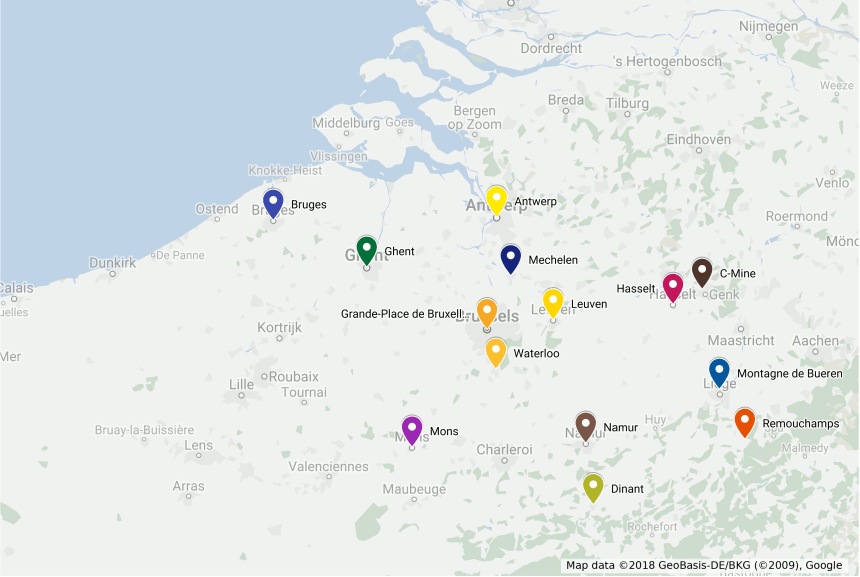
\includegraphics[width=0.6\textwidth]{../images/belgium-tourism-14.png}
		\par\end{centering}
	\caption{14 cidades turísticas da Bélgica}	
	\label{figG}
\end{figure}


\subsection{Uma Formulação Compacta}

O problema do caixeiro viajante pode ser modelado utilizando-se uma
formulação compacta, isto é, uma formulação com um número polinomial
de variáveis e restrições. Formulações desse tipo, apesar de usualmente não serem a melhor opção de resolução em termos de desempenho para problemas
deste tipo, são convenientes para uma primeira abordagem pois podem
ser facilmente inseridas de uma vez só como entrada para um software
resolvedor. A formulação abaixo foi proposta por \cite{Miller1960}:

\begin{align}
    \textrm{Minimize: }   & \nonumber \\
    &  \sum_{i \in I, j \in I} c_{i,j} \ldotp x_{i,j} \\
    \textrm{Sujeito a: }   & \nonumber \\
    & \sum_{j \in V \setminus \{i\}} x_{i,j} = 1 \,\,\, \forall i \in V \label{eq:in}  \\
    & \sum_{i \in V \setminus \{j\}} x_{i,j} = 1 \,\,\, \forall j \in V \label{eq:out} \\
    & y_{i} -(n+1)\ldotp x_{i,j} \geq y_{j} -n  \,\,\, \forall i \in V\setminus \{0\}, j \in V\setminus \{0,i\} \label{eq:st1} \\
    & x_{i,j} \in \{0,1\} \,\,\, \forall i \in V, j \in V \\
    & y_i \geq 0 \,\,\, \forall i \in V 
\end{align}

As equações (\ref{eq:in}) e (\ref{eq:out}) garantem que cada vértice
é visitado somente uma vez enquanto variáveis auxiliares $y_{i}$
são utilizadas nas restrições (\ref{eq:st1}) para garantir que uma vez
que um arco $(i,j)$ seja selecionado, o valor de $y_{j}$ seja maior
do que o valor de $y_{i}$ em uma unidade. Essa propriedade é garantida
para todos os vértices exceto o vértice 0 que é arbitrariamente selecionado
como origem de modo a evitar a construção de sub-rotas desconectadas,
como no exemplo da Figura \ref{figSub}, onde os valores das variáveis
$x_{(i,j)}$ indicados nos arcos representam uma solução viável caso
somente as restrições (\ref{eq:in}) e (\ref{eq:out}) fossem consideradas.

\begin{figure}
	\begin{centering}
		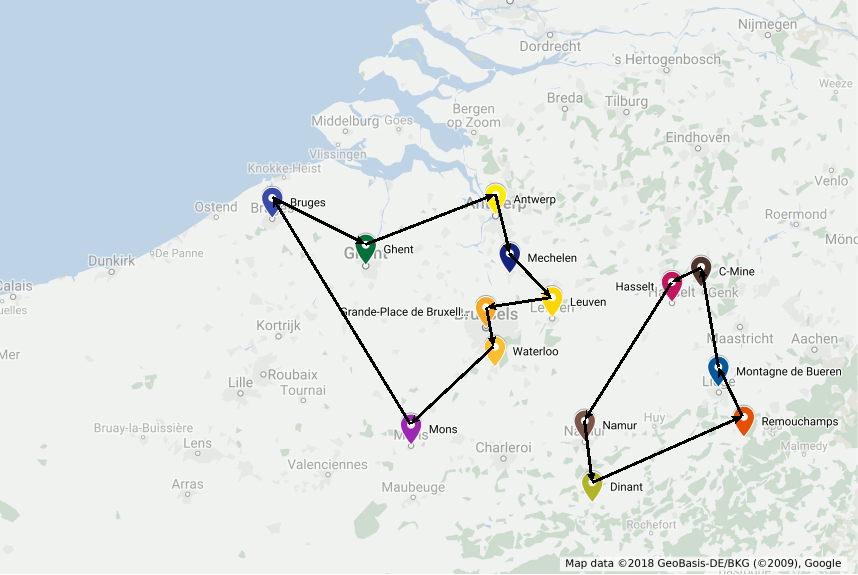
\includegraphics[width=0.6\textwidth]{belgium-tourism-14-subtour.png}
		\par\end{centering}
	\caption{Rotas desconectadas da origem}
	\label{figSub}
	
\end{figure}

A seguir temos um exemplo completo de um resolvedor em Python-MIP para o problema do caixeiro viajante para o mapa Figura \ref{figG}, onde o resolvedor utilizará a formulação compacta descrita anteriormente:

{\small
\lstinputlisting[breaklines]{tsp-compact.py}
}

Nas linhas 6-9 nomeamos nossos pontos turísticos. Nas linhas 12-25 informamos o tempo estimado de deslocamento entre cada par de cidades $(i, j)$ onde $i<j$, visto que em nosso exemplo consideramos que a distância de ida e volta é igual. Convertemos a matriz triangular \texttt{dists} em uma matriz completa nas linhas 31-34.

A linha 36 cria o modelo de programação linear inteira. As variáveis do modelo são criadas nas linhas 39 e 42 utilizando o método \texttt{add\_var} em nosso modelo \texttt{m}. Durante a criação das restrições, será necessário referenciar as variáveis criadas. Por isso, utilizamos a matriz \texttt{x} para mapear cada arco do grafo com sua respectiva variável binária e  vetor \texttt{y} para mapear cada nó com sua respectiva variável auxiliar contínua para eliminação de sub-rotas.

A função objetivo que minimiza o tempo total dos arcos selecionados é informada na linha 45. Nesse caso, para cada arco multiplicamos sua respectiva variável binária de seleção pelo tempoo de deslocamento do arco armazenado em \texttt{c}.

As restrições são criadas nas linhas 48-57. Em todos os casos utilizamos o operador \texttt{+=} sobre o modelo \texttt{m} para adicionar restrições lineares. Note que assim como na função objetivo, o somatório é efetuado com a função \texttt{xsum}. Esta função é similar a função \texttt{sum} disponível na linguagem Python mas otimizada para a situação específica de escrita de restrições lineares no pacote Python-MIP\@. 

A linha 60 dispara a otimização do modelo. Na linha 63 verificamos se uma solução viável foi encontrada e se positivo a escrevemos nas linhas 64-72.

Os resolvedores de programação linear inteira executam uma busca em árvore onde são utilizados limites para a poda de nós. O limite superior é obtido a partir de qualquer solução viável que for encontrada durante a busca e o limite inferior corresponde ao custo obtido com a resolução do problema com as restrições de integralidade das variáveis relaxadas. No nosso caso considerando domínio das variáveis $x$ como contínuo entre 0 e 1. A formulação aqui utilizada tem uma grave deficiência: o limite inferior por ela produzido é distante do custo ótimo da solução. Desse modo, o desempenho dos resolvedores de programação linear inteira em sua resolução é bastante pobre. Essa deficiência não é visível quando resolvemos problemas pequenos como o de exemplo (apenas 14 cidades), mas faz com que o desempenho do resolvedor degenere muito rapidamente a medida que o tamanho do grafo de entrada aumenta.


\subsection{Tratamento de Formulações Fortes com Geração Dinâmica de Restrições}

A formulação do caixeiro viajante utilizada nos resolvedores de melhor desempenho inclui restrições de eliminação de sub-rotas do tipo:

\begin{equation}
	\sum_{(i,j) \in S \times S} x_{(i,j)} \leq |S|-1 \,\,\, \forall S \subset V 
\end{equation}

O problema com as desigualdades acima é que elas devem ser geradas para \emph{cada subconjunto} $S$ de vértices do grafo, ou seja, para uma grafo com $n$ vértices temos $2^n-1$ subconjuntos não vazios. Inseri-las no modelo inicial é inviável exceto para instâncias pequenas. Uma solução para esse problema é o método dos planos de corte \citep{Dantzig54}, onde somente as restrições \emph{necessárias} são inseridas. O pacote Python-MIP permite uma comunicação bi-direcional com o resolvedor para que as restrições necessárias sejam inseridas \emph{durante} a busca. Para isso precisamos criar uma classe derivada da classe \texttt{ConstrsGenerator} que implemente o método \texttt{generate\_constrs}. Esse método recebe como parâmetro um modelo, onde a solução corrente pode ser consultada e restrições adicionais podem ser inseridas na medida do necessário. 

O pacote Python-MIP permite um controle sobre em que ponto da busca as restrições faltantes serão verificadas. Duas propriedades do modelo podem ser preenchidas com objeto(s) do tipo \texttt{ConstrsGenerator}:

\begin{description}
	\item[\texttt{cuts\_generator}]: caso o gerador de restrições seja informado nessa propriedade do modelo, a verificação por restrições faltantes (cortes violados) será realizada sempre que uma \emph{solução fracionária} for gerada durante a resolução de um nó na árvore de busca. Nesse caso, cortes são inseridos para \emph{reforçar} a formulação inserida inicialmente, ou seja, caso somente um \texttt{cuts\_generator} seja informado é necessário que a formulação inicial seja completa; assim, caso a restrição (7) seja inserida dessa forma, as variáveis auxiliares $y$ e as restrições (fracas) de eliminação de sub-ciclos devem ser mantidas na formulação inicial.
	
	\item[\texttt{lazy\_constrs\_generator}]: um gerador de restrições informado nessa propriedade será chamado sempre que uma \emph{solução inteira} for gerada. Nesse modo de uso é possível iniciar a busca com uma formulação incompleta, ou seja, sem as variáveis auxiliares $y$ e as restrições (4). Desse modo, a formulação inicial pode ficar muito mais leve. Uma possível desvantagem desta abordagem é que como o resolvedor deve considerar que a formulação inicial está incompleta, algumas fases do pré-processamento do mesmo precisam ser desligadas e o limite inferior inicial pode ser menor.
\end{description}

Uma vez que tenhamos um gerador de restrições implementado, podemos decidir em que situação o mesmo será chamado. É possível também especificar geradores de restrições para ambas as situações, ou seja, a formulação inicial será incompleta e portanto toda solução inteira deve ser checada mas soluções fracionárias também serão checadas. A melhor abordagem a ser utilizada deve ser determinada com experimentos no problema de interesse.


Em soluções inteiras como a da Figura 2, a identificação de sub-rotas pode ser facilmente realizada executando-se uma busca em profundidade a partir de cada nó e verificando sua conectividade. A existência ou não de um arco depende do valor da respectiva variável $x$ na solução inteira.

O código abaixo implementa um gerador dinâmico de restrições de eliminação de sub-rotas em soluções inteiras para nossa formulação compacta previamente implementada. 

{\small
\begin{lstlisting}
from mip.callbacks import ConstrsGenerator, CutPool
from typing import Set, List
from collections import defaultdict

def subtour(N: Set, out: defaultdict, node) -> List:
    """verifica se 'node' pertence a uma sub-rota. 
    se positivo retorna os elementos dessa sub-rota"""
    queue = [node]
    visited = set(queue)
    while queue:
        n = queue.pop()
        for nl in out[n]:
            if nl not in visited:
                queue.append(nl)
                visited.add(nl)

    if len(visited) != len(N):
        return [v for v in visited]
    else:
        return []

class SubTourLazyGenerator(ConstrsGenerator):
    """Gera restrições de eliminação de sub-rotas em soluções inteiras"""
    def generate_constrs(self, model: Model):
        r = [(v, v.x) for v in model.vars
             if v.name.startswith('x(') and v.x >= 0.99]
        U = [int(v.name.split('(')[1].split(',')[0]) for v, f in r]
        V = [int(v.name.split(')')[0].split(',')[1]) for v, f in r]
        N, cp = set(U+V), CutPool()
        # output nodes for each node
        out = defaultdict(lambda: list())
        for i in range(len(U)):
            out[U[i]].append(V[i])

        for n in N:
            S = set(subtour(N, out, n))
            if S:
                arcsInS = [(v, f) for i, (v, f) in enumerate(r)
                           if U[i] in S and V[i] in S]
                if sum(f for v, f in arcsInS) >= (len(S)-1)+1e-4:
                    cut = xsum(1.0*v for v, fm in arcsInS) <= len(S)-1
                    cp.add(cut)
        for cut in cp.cuts:
            model += cut
\end{lstlisting}
}

Para que esse código seja executado durante a busca, antes de chamar a otimização do modelo no código anterior (linha 60), precisamos informar o gerador atribuindo um objeto desse tipo à propriedade \texttt{lazy\_constrs\_generator} com o código: 

\begin{center}
\texttt{model.lazy\_constrs\_generator = SubTourLazyGenerator()}
\end{center}

A versão completa do código que inclui a geração dinâmica de restrições de eliminação de sub-rotas em soluções inteiras pode ser baixada no seguinte endereço: \url{https://raw.githubusercontent.com/coin-or/python-mip/master/docs/podes/tsp-lazy.py} .

A geração de desigualdades que eliminam soluções fracionárias determina o problema conhecido como \emph{separação de cortes}. No nosso caso queremos encontrar sub-conjuntos de vértices pouco conectados ao restante da rota. Esse problema pode ser resolvido solucionando-se o problema do corte mínimo considerando o grafo da malha viária do problema com o valor das variáveis $x$ como capacidades nos arcos.
Em nosso exemplo utilizaremos a implementação do algoritmo de corte mínimo disponível no pacote Python \texttt{networkx}.

{\small
\begin{lstlisting}
import networkx as nx

class SubTourCutGenerator(ConstrsGenerator):
    def __init__(self, Fl: List[Tuple[int, int]]):
        self.F = Fl

    def generate_constrs(self, model: Model):
        G = nx.DiGraph()
        r = [(v, v.x) for v in model.vars if v.name.startswith('x(')]
        U = [int(v.name.split('(')[1].split(',')[0]) for v, f in r]
        V = [int(v.name.split(')')[0].split(',')[1]) for v, f in r]
        cp = CutPool()
        for i in range(len(U)):
            G.add_edge(U[i], V[i], capacity=r[i][1])
        for (u, v) in F:
            if u not in U or v not in V:
                continue
            val, (S, NS) = nx.minimum_cut(G, u, v)
            if val <= 0.99:
                arcsInS = [(v, f) for i, (v, f) in enumerate(r)
                           if U[i] in S and V[i] in S]
                if sum(f for v, f in arcsInS) >= (len(S)-1)+1e-4:
                    cut = xsum(1.0*v for v, fm in arcsInS) <= len(S)-1
                    cp.add(cut)
                    if len(cp.cuts) > 256:
                        for cut in cp.cuts:
                            model += cut
                        return
        for cut in cp.cuts:
            model += cut
        return
\end{lstlisting}}

Na criação de nosso gerador de cortes informamos uma lista \texttt{Fl} de pares $(i,j)$ de vértices cuja conectividade deve ser checada em toda solução gerada. No método \texttt{generate\_constrs} consultamos as variáveis do modelo (\texttt{model.vars}) e identificamos a qual arco cada variável se refere considerando o nome das variáveis (linhas 9-11), utilizando o seu valor na solução (propriedade \texttt{x}) para construção do grafo onde iremos procurar sub-rotas desconexas para geração das restrições (6). A descoberta de sub-rotas desconexas (linhas 19) gera a restrição de restrições (cortes) que são primeiramente armazenados em um conjunto (linha 24) e posteriormente adicionados ao modelo. Separamos esses dois passos pois restrições repetidas podem ser geradas. Na linha 25 inserimos um critério de parada para a geração dos cortes: caso um número suficientemente grande já tenha sido gerado, inserimos os mesmos no modelo e prosseguimos a otimização sem procurar por cortes adicionais. Nesse ponto convém ressaltar a função dos cortes e sua relação com o restante do modelo. Como a formulação compacta que estamos utilizando define completamente o problema, a adição de cortes é opcional, ou seja, somente feita para melhorar o desempenho do modelo. A inserção de um número muito grande de cortes por iteração pode gerar o efeito indesejado de perda de desempenho na resolução. Para utilizamos nosso gerador de cortes com a formulação anterior basta atribuir à propriedade \texttt{cuts\_generator} um objeto da nossa classe \texttt{SubTourCutGenerator} antes da otimização do modelo.

\subsection{Integração com heurísticas}

Resolvedores de programação linear inteira iniciam o processo de resolução computando uma solução possivelmente fracionária, obtida através da relaxação do problema. Em instâncias difíceis, a obtenção da primeira solução \emph{inteira} válida pode requerer a exploração de um grande número de nós na árvore de busca. Para essas instâncias, muitas vezes uma heurística simples e rápida pode ser utilizada para geração de uma solução inicial. No pacote Python-MIP soluções iniciais podem ser facilmente informadas ao resolvedor através da propriedade \texttt{start} do modelo que recebe uma lista de pares \texttt{(x, v)} onde \texttt{x} é uma referência para uma variável de decisão e \texttt{v} o seu valor na solução factível. 

O código abaixo demonstra a utilização de um algoritmo construtivo e de uma metaheurística de busca local para construção de uma solução inicial factível para nosso modelo.
 
{\small
\begin{lstlisting}
seq = [0, max((c[0][j], j) for j in V)[1]] + [0]
Vout = V-set(seq)
while Vout:
    (j, p) = min([(c[seq[p]][j] + c[j][seq[p+1]], (j, p)) for j, p in
                  product(Vout, range(len(seq)-1))])[1]

    seq = seq[:p+1]+[j]+seq[p+1:]    
    Vout = Vout - {j}


def delta(d: List[List[float]], S: List[int], p1: int, p2: int) -> float:
    p1, p2 = min(p1, p2), max(p1, p2)
    e1, e2 = S[p1], S[p2]
    if p1 == p2:
        return 0
    elif abs(p1-p2) == 1:
        return ((d[S[p1-1]][e2] + d[e2][e1] + d[e1][S[p2+1]])
                - (d[S[p1-1]][e1] + d[e1][e2] + d[e2][S[p2+1]]))
    else:
        return (
        (d[S[p1-1]][e2] + d[e2][S[p1+1]] + d[S[p2-1]][e1] + d[e1][S[p2+1]])
        - (d[S[p1-1]][e1] + d[e1][S[p1+1]] + d[S[p2-1]][e2] + d[e2][S[p2+1]]))

L = [cost for i in range(50)]
sl, cur_cost, best = seq.copy(), cost, cost
for it in range(int(1e7)):
    (i, j) = rnd.randint(1, len(sl)-2), rnd.randint(1, len(sl)-2)
    dlt = delta(c, sl, i, j)
    if cur_cost + dlt <= L[it % len(L)]:
        sl[i], sl[j], cur_cost = sl[j], sl[i], cur_cost + dlt
        if cur_cost < best:
            seq, best = sl.copy(), cur_cost
    L[it % len(L)] = cur_cost
    
m.start = [(x[seq[i]][seq[i+1]], 1) for i in range(len(seq)-1)]    
\end{lstlisting}}

Nosso algoritmo construtivo (linhas 262-269) será o algoritmo da inserção mais barata: dada uma rota que não inclua todos as cidades, na inserção de uma nova cidade verificamos o custo de inserir cada cidade ainda fora da rota (elemento \texttt{j} conjunto \texttt{Vout} em cada posição intermediária possível (\texttt{p}) e selecionamos a opção mais barata.

Para melhoria da nossa solução inicial utilizaremos a metaheurística baseada em busca local Late Acceptance Hill Climbing \citep{burke2017} por sua simplicidade. O gargalo de métodos de busca local usualmente é a avaliação do custo da solução resultante da aplicação de dado movimento. Por isso, nas linhas 11-22 incluímos uma função que dada uma solução de entrada (sequência de cidades) \texttt{s} e duas posições dessa sequência, \texttt{p1} e \texttt{p2} calcula em \emph{tempo constante} a variação de custo que será obtida. Dessa forma, podemos executar rapidamente um grande número de movimentos cuja aceitação é controlada pelo arcabouço da metaheurística que é implementada nas linhas 25-33. Finalmente, informamos as variáveis de decisão relacionadas aos arcos existentes na melhor solução encontrada na linha 35.


		
\bibliography{pmip-podes}
\bibliographystyle{podes-bibstyle}


\end{document}
